\chapter{Installation}

PARALUTION can be compiled under Linux/Unix, Windows and Mac operating systems.

\textbf{\emph{Note}} Please check Section~\ref{remark-compilation} for additional remarks.

\section{Linux/Unix-like OS}
After downloading and unpacking the library, the user needs to compile it. We provide two compilation configurations -- \emph{cmake} and \emph{Makefile}.

\subsection{Makefile}
In this case, the user needs to modify the Makefile which contains the information about the available compilers. By default PARALUTION will only use gcc \cite{gcc} compiler (no GPU support). The user can switch to icc \cite{icc} with or without MKL \cite{mkl} support. To compile with GPU support, the user needs to uncomment the corresponding CUDA\footnote{NVIDIA CUDA, when mentioned  also includes CUBLAS and CUSPARSE} \cite{cuda} lines in the Makefile. The same procedure needs to be followed for the OpenCL \cite{opencl} and for the OpenMP(MIC) backend. 

\textbf{\emph{Note}} During the compilation only one backend can be selected, i.e. if a GPU is available the user needs to select either CUDA or OpenCL support. 

The default installation process can be summarized in the following lines:
\lstinputlisting{./src/get_install_paralution.sh}
where {x.y.z} is the version of the library. 

\textbf{\emph{Note}} Please note, that the multi-node version of PARALUTION can only be compiled using CMake.


\subsection{CMake}
The compilation with cmake \cite{cmake} is easier to handle -- all compiler specifications are determined automatically. 

The compilation process can be performed by
\lstinputlisting{./src/get_install_paralution_cmake.sh}
where {x.y.z} is the version of the library. Advanced compilation can be performed with \emph{cmake -i ..}, you need this option to compile the library with OpenMP(MIC) backend.

The priority during the compilation process of the backends are: CUDA, OpenCL, MIC

You can also choose specific options via the command line, for example CUDA:
\lstinputlisting{./src/cmake2.sh}

For the Intel Xeon Phi, OpenMP(MIC) backend with MPI support:
\lstinputlisting{./src/cmake3.sh}

\textbf{\emph{Note}} ptk file is generated in the build directory when using cmake.

\subsection{Shared Library}
Both compilation processes produce a shared library file \emph{libparalution.so}. Ensure that the library object can be found in your library path. If you do not copy the library to a specific location you can add the path under Linux in the \emph{LD\_LIBRARY\_PATH} variable.
\lstinputlisting{./src/shared_lib.txt}


\section{Windows OS}

This section will introduce a step-by-step guide to compile and use the PARALUTION library in a Windows based environment.
\textbf{\emph{Note}} Please note, that the multi-node version does not support Windows/Visual Studio.

\subsection{OpenMP backend}

PARALUTION with OpenMP backend comes with Visual Studio Project files that support Visual Studio 2012 and 2013. PARALUTION is built as a static library during this step-by-step guide.

\begin{itemize}

  \item Open Visual Studio and navigate to \emph{File\textbackslash Open Project}.
  \begin{figure}[!ht]
  \centering
  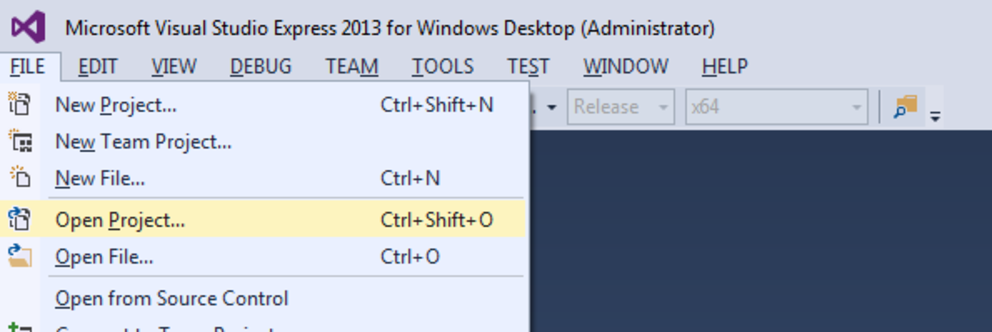
\includegraphics[width=0.5\textwidth]{./fig/visualstudio/vs_1.pdf}
  \caption{Open an existing Visual Studio project.}
  \label{vs1}
  \end{figure}

  \item Load the corresponding PARALUTION project file, located in the \emph{visualstudio\textbackslash paralution\_omp} directory. The \emph{PARALUTION} and \emph{CG} projects should appear.
  \begin{figure}[!ht]
  \centering
  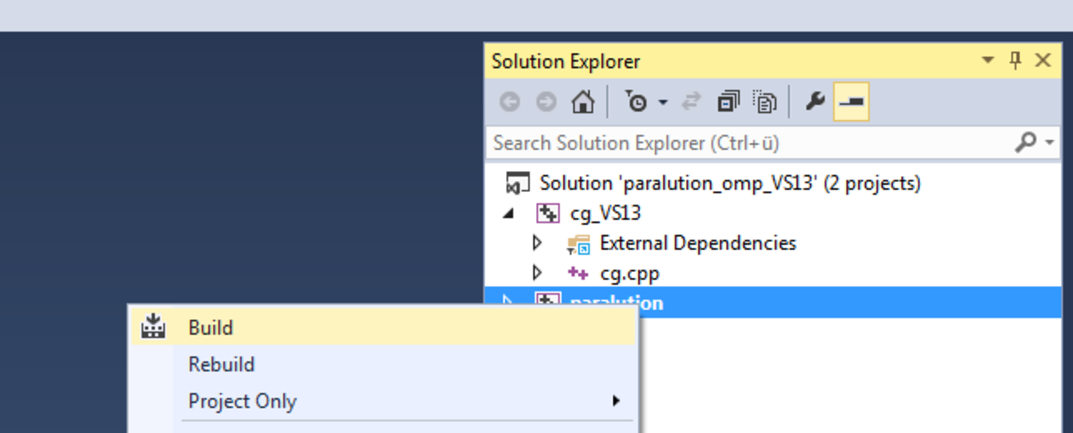
\includegraphics[width=0.5\textwidth]{./fig/visualstudio/vs_2.pdf}
  \caption{Build the PARALUTION library.}
  \label{vs2}
  \end{figure}

  \item Right-click the \emph{PARALUTION} project, and start to build the library. Once finished, Visual Studio should report a successful built.
  \begin{figure}[!ht]
  \centering
  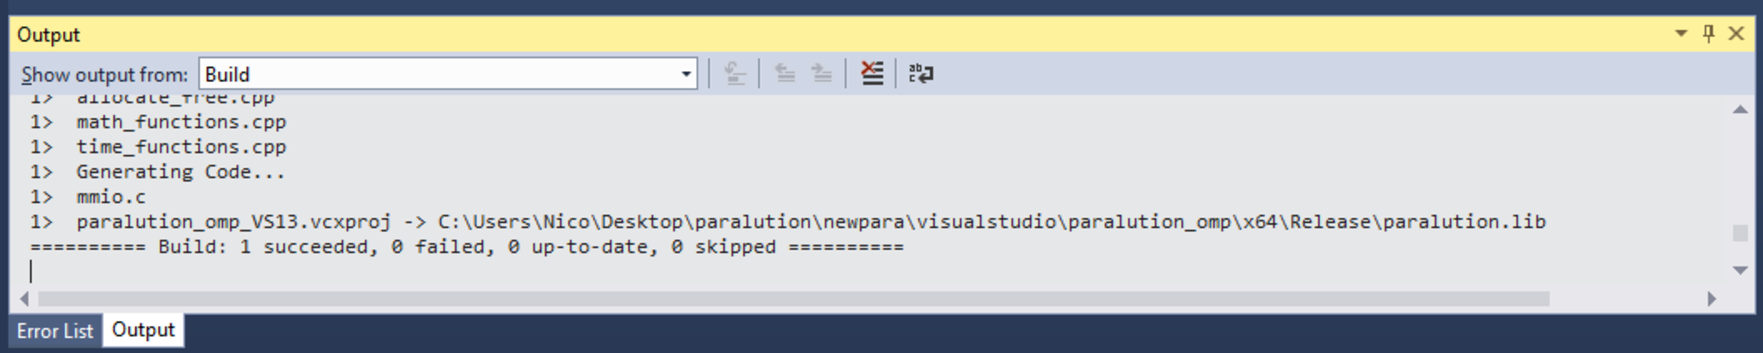
\includegraphics[width=1.0\textwidth]{./fig/visualstudio/vs_3.pdf}
  \caption{Visual Studio output for a successful built of the static PARALUTION library.}
  \label{vs3}
  \end{figure}

  \item Next, repeat the building procedure with the \emph{CG} example project. Once finished, a successful built should be reported.
  \begin{figure}[!ht]
  \centering
  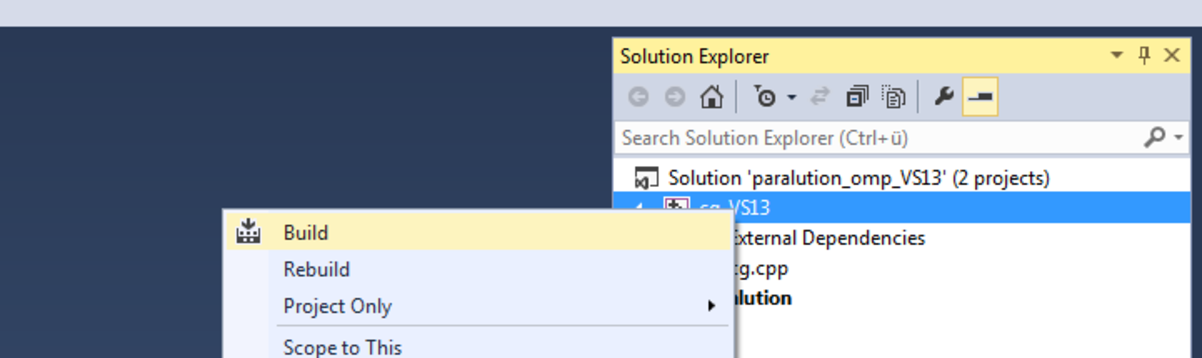
\includegraphics[width=0.5\textwidth]{./fig/visualstudio/vs_4.pdf}
  \caption{Build the PARALUTION CG example.}
  \label{vs4}
  \end{figure}

  \item Finally, the \emph{CG} executable should be located within the \emph{visualstudio\textbackslash paralution\_omp\textbackslash Release} directory.  
  \begin{figure}[!ht]
  \centering
  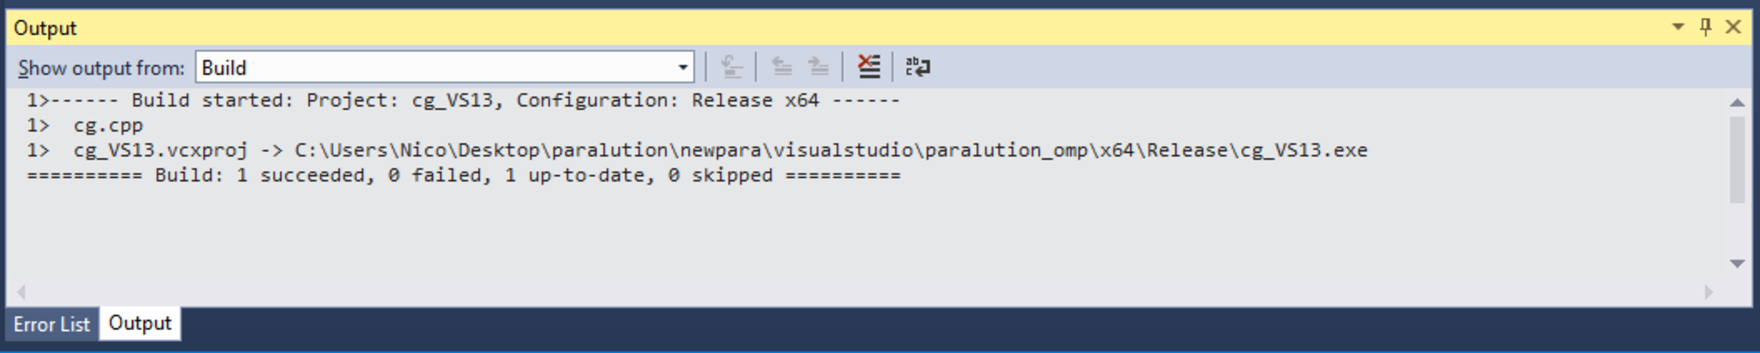
\includegraphics[width=1.0\textwidth]{./fig/visualstudio/vs_5.pdf}
  \caption{Visual Studio output for a successful built of the PARALUTION CG example.}
  \label{vs5}
  \end{figure}

\end{itemize}

\textbf{\emph{Note}} For testing, Windows 7 and Visual Studio Express 2013 has been used.

\textbf{\emph{Note}} OpenMP support can be enabled/disabled in the project properties. Navigate to \emph{C++\textbackslash Language} for the corresponding switch.

\textbf{\emph{Note}} For MPI support, the Microsoft MPI SDK has to be installed.


\subsection{CUDA backend}

PARALUTION with CUDA backend comes with Visual Studio Project files that support Visual Studio 2012 and 2013. Please follow the same steps as for the OpenMP backend compilation but using the \emph{visualstudio\textbackslash paralution\_cuda} directory.

\subsection{OpenCL backend}

PARALUTION with OpenCL backend comes with Visual Studio Project files that support Visual Studio 2012 and 2013. Please follow the same steps as for the OpenMP backend compilation but using the \emph{visualstudio\textbackslash paralution\_ocl} directory. Additionally, the OpenCL include directory and OpenCL library directory need to be specified within Visual Studio, as illustrated in Figures~\ref{ocl_inc}~and~\ref{ocl_lib}.

\begin{figure}[!ht]
\centering
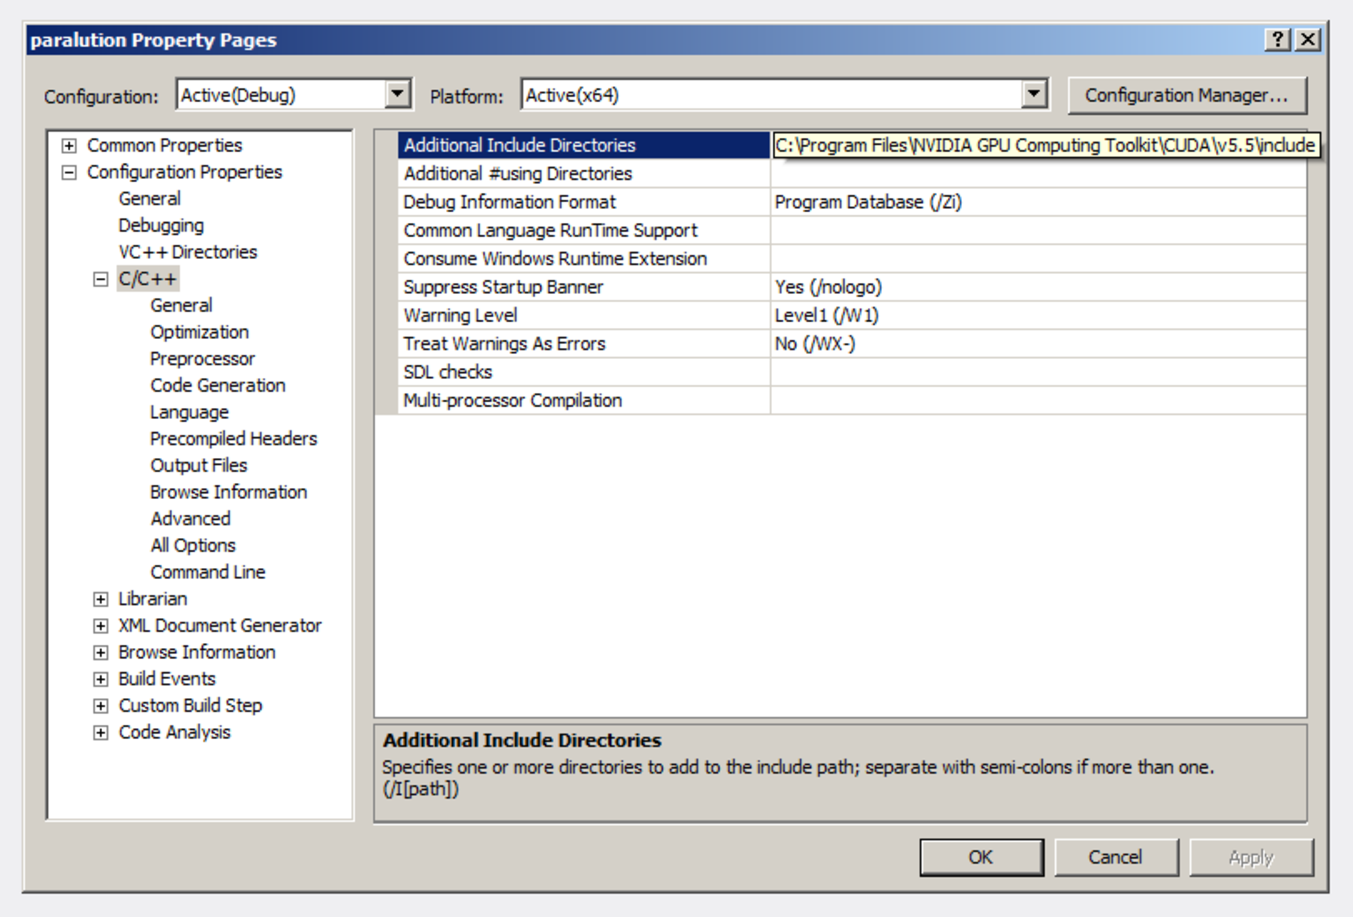
\includegraphics[width=0.9\textwidth]{./fig/visualstudio/ocl_include.pdf}
\caption{Setting up Visual Studio OpenCL include directory.}
\label{ocl_inc}
\end{figure}

\begin{figure}[!ht]
\centering
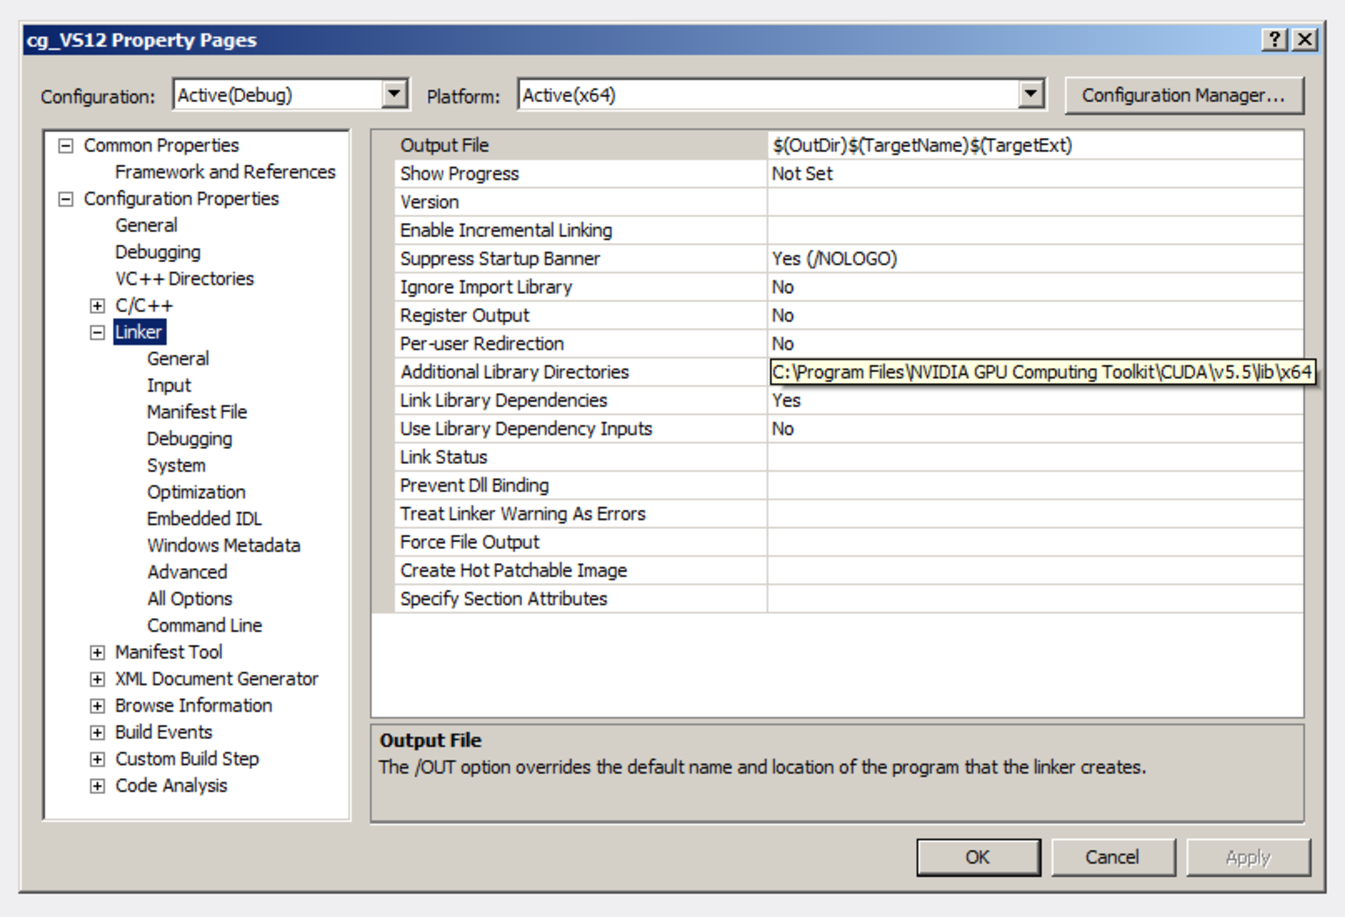
\includegraphics[width=0.9\textwidth]{./fig/visualstudio/ocl_lib.pdf}
\caption{Setting up Visual Studio OpenCL library directory.}
\label{ocl_lib}
\end{figure}

\section{Mac OS}

To compile PARALUTION under Mac, please follow the Linux/Unix-like OS instruction for the \emph{CMake} compilation.

\section{Supported Compilers}

The library has been tested with the following compilers: 

\begin{table}[!h]
  \centering
\begin{tabular}{ l l l }
    \hline
  cmake & 2.8.12.2; 3.0.2; 3.1.3; 3.2.0 & S,M \\
    \hline
  gcc/g++ & 4.4.7; 4.6.3; 4.8.2, 4.8.5 & S,M \\
    \hline
  icc (MKL) & 12.0; 13.1; 14.0.4; 15.0.0 & S,M \\
    \hline
  CUDA & 5.0; 5.5; 6.0; 6.5; 7.0; 7.5  & S,M \\
    \hline
  Intel OpenCL  & 1.2 & S,M \\
    \hline
  NVIDIA OpenCL  & 1.2 & S,M \\
    \hline
  AMD OpenCL  & 1.2; 2.0 & S,M \\
    \hline
  Visual Studio  & 2012, 2013 & S,M \\
    \hline
  MPICH       & 3.1.3 & M \\
  OpenMPI      & 1.5.3; 1.6.3; 1.6.5; 1.8.4 & M \\
  Intel MPI   & 4.1.2; 5.0.1 & M \\
    \hline

\end{tabular}
\end{table}

\textbf{\emph{Note}} Please note, that CUDA has limited ICC support. \\
\textbf{\emph{Note}} Please note, that Intel MPI \textgreater = 5.0.0 is only supported by CMAKE \textgreater = 3.2.0.


\section{Simple Test}
You can test the installation by running a CG solver on a Laplace matrix \cite{gr3030}. After compiling the library you can perform the CG solver test by executing:
\lstinputlisting{./src/download_test_cg.sh}


\section{Compilation and Linking}

After compiling the PARALUTION library, the user need to specify the include and the linker path to compile a program.

\lstinputlisting[title="Compilation and linking"]{./src/compilation.sh}

Before the execution of a program which has been compiled with PARALUTION, the library path need to be added to the environment variables, similar to
\lstinputlisting{./src/shared_lib.txt}

When compiling with MPI, library and program need to be compiled using \emph{mpic++} or the corresponding MPI C++ compiler.
